
\section{Infrastructure Nextcloud}
\subsection{L'architecture}
\begin{frame}{L'architecture}
\vspace{-50pt}
\begin{figure}
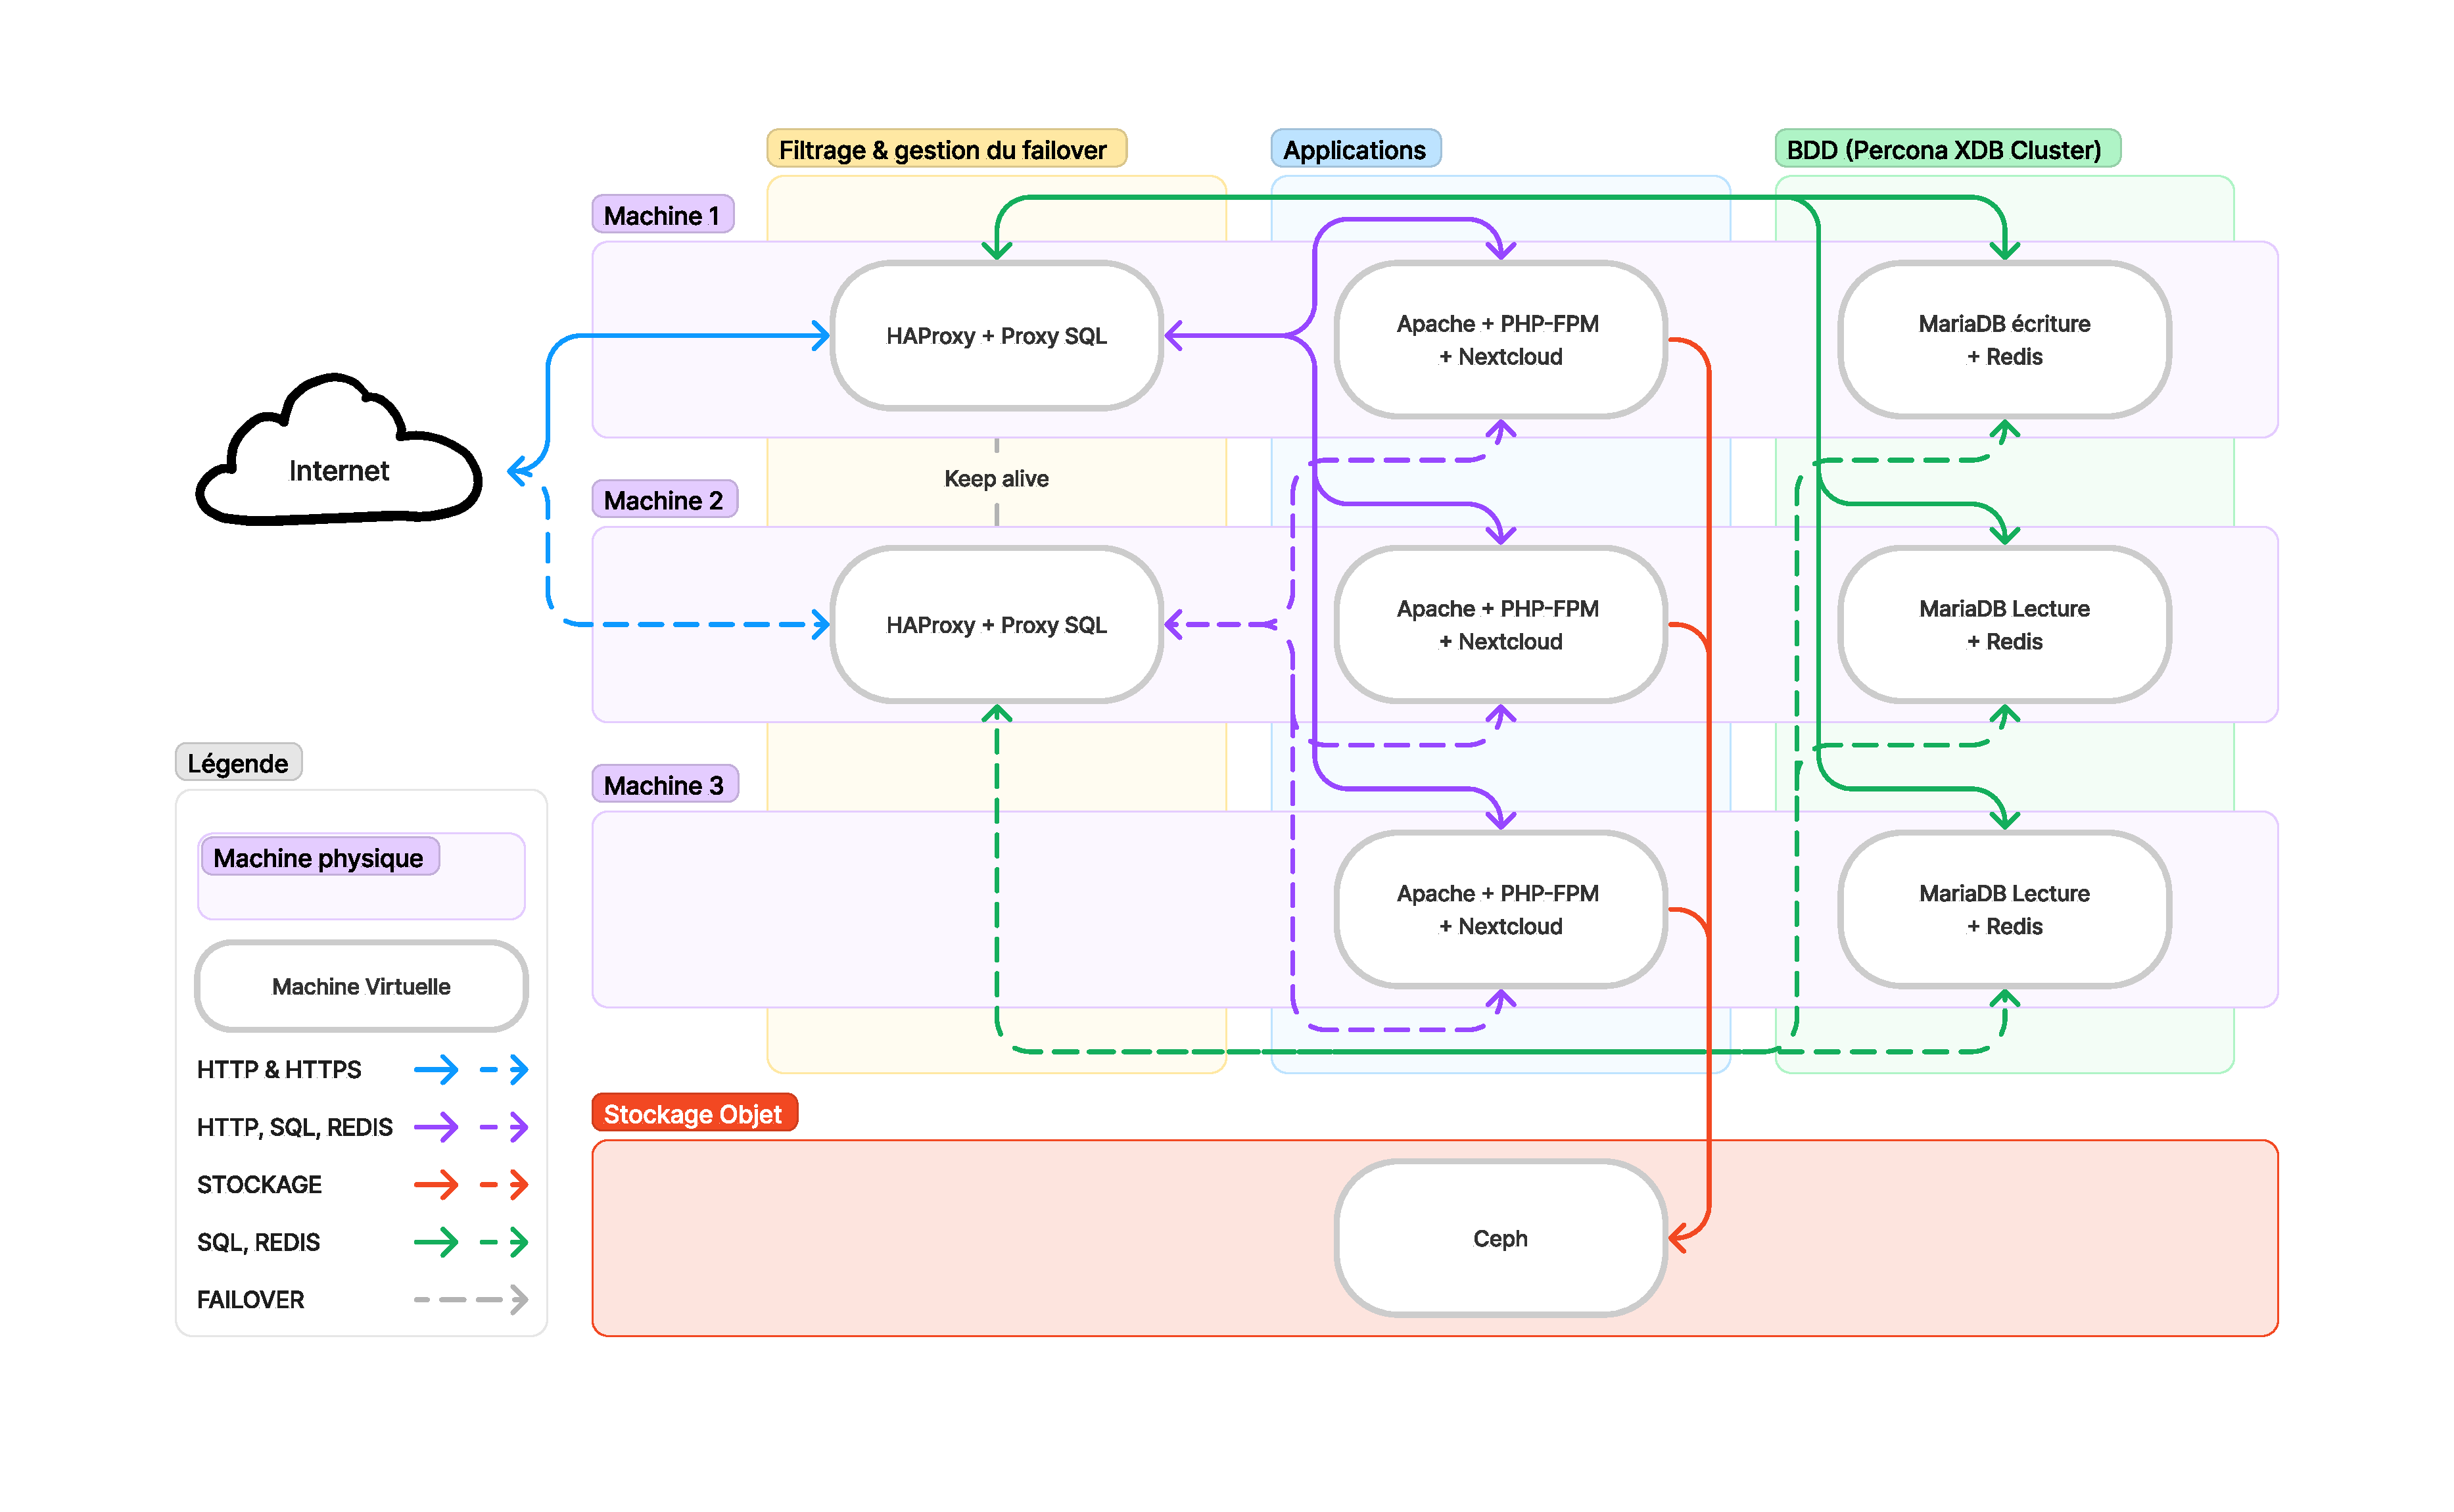
\includegraphics[scale=0.25]{202306-architecture-nextcloud.pdf}
\end{figure}
\end{frame}

\subsection{Les instances de production}
\begin{frame}{Les instances de production} 
Deux instances de production sur la même infrastructure.
\begin{enumerate}
	\item Pour l'ENT depuis mai 2020 (V18.0.3 ... V24.0.12)
		\begin{list}{-}{}
		  \item $9$ domaines (avec leurs css)
		  \item $372$ établissements;
		  \item $118\,224$ comptes actifs;
		  \item $67\,383$ groupes;
		  \item Création des comptes et groupes automatique depuis LDAP;
		 \end{list}

	\item Pour le Gip Recia (V25.0.6) (extension aux collectivités locales?) 
	   \begin{list}{-}{}
	   \item Stockage NetApp.
	   \item Création  automatique des comptes, groupes et  groupFolder;
	   \end{list}
\end{enumerate}
\end{frame}
